% Toolbar icon: transferField — conservative field transfer between meshes. Two
% grids of different resolution with an arrow from the coarse one to the fine
% one: the operation moves DATA between discretizations, and the differing cell
% sizes are the whole point (identical meshes would need no transfer).
% Distinct from `mergeMesh` (two bodies becoming one) — here both stay, and only
% values cross.
\documentclass[tikz,border=2mm]{standalone}
\usetikzlibrary{arrows.meta,calc,shapes.geometric}
\begin{document}
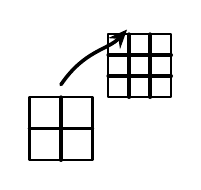
\begin{tikzpicture}[line width=1.3pt, line cap=round, line join=round, x=1mm,y=1mm]
  % Source: coarse 2x2.
  \draw[thick] (-9,-8) rectangle (-1,0);
  \draw (-5,-8) -- (-5,0);
  \draw (-9,-4) -- (-1,-4);
  % Target: fine 3x3.
  \draw[thick] (1,0) rectangle (9,8);
  \foreach \d in {2.667,5.333} {
    \draw (1+\d,0) -- (1+\d,8);
    \draw (1,\d) -- (9,\d);
  }
  % The transfer.
  \draw[-{Stealth[length=2.4mm,width=2.0mm]}] (-5,1.6) .. controls (-2,6) and (1,6) .. (3.4,8.6);
\end{tikzpicture}
\end{document}
